\section{DemoInfo module}
This module store the textual description of the demo and allows to ask for specific sections of it. It also stores other demo-related information, as:
\begin{itemize}
\item Demo id
\item Abstract
\item Title 
\item Authors list
\item Authors email list
\item Article URL
\item State (inactive,preprint, published)
\item Demo editor
\item Demo editor email
\item Demo zip file containing demo DDL 
\item Demo DDL JSON
\end{itemize}

\subsection{DemoInfo module structure}
This Module is made of:
\begin{itemize}
\item model.py where the db structure, the DAO (Data access object) classes and some helper classes (Demo, Author and Editor) are defined. It provides a layer of abstraction over the DB.
\item demoinfo.conf it's the cherrypy config for the webservices module.
\item demoinfo.py it's the webservices module.
\item testdemoinfo.py it's the tests to check that the webservices work.
\item testdemoinfo.conf it's the cherrypy config for testing.
\end{itemize}

\subsection{The model (database) structure}
The model of this module id made of the following tables:

\begin{figure}[!ht]
\centering
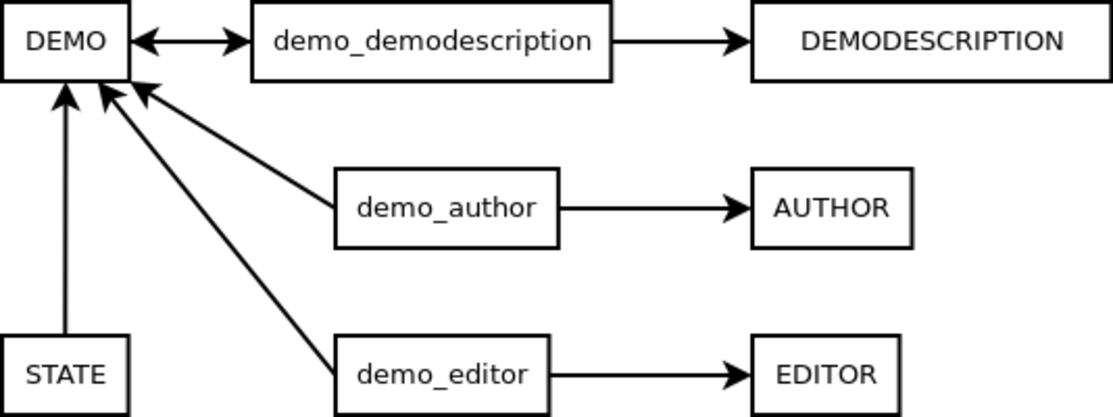
\includegraphics[width=0.8\linewidth]{demo_info/images/demoinfo_model.pdf}
\caption{Demoinfo Database Model. \miguel{Let's avoid having non-generated figures. If we do so, we're forced to redraw the figures by hand, instead of simply recreating them from the data. [ToDo] Look for a tool which creates automatically vectorial graphics from the data.}} 
\label{fig:demoinfo_model}
\end{figure}

Note that states is the table for the demo's state (published, preprint, \dots)
The Demodescription table is where the DDL of each demo is stored.
A demo may be created without a DDL (but you will need to provide one so you can run it)
Ddlschema is not used at the moment, but it has been created so that a schema validation can be done to the DDL of each demo, if a user provides a valid json for the DDL but this json is not a valid DDL, we should be able to detect this and return an error.

\subsection{Web services available}
This module provides a set of webservices, those that return data can be called with GET or other HTML methods, those that delete,create or update data can be called only by POST.
These webservices are shown grouped by functionality, 

DEMO

\begin{itemize}
\item  demo\_list(self)
\item  demo\_list\_by\_demoeditorid(self,demoeditorid\_list)
\item  demo\_list\_pagination\_and\_filter(self,number\_elements\_page,page,qfilter=None)
\item  demo\_get\_authors\_list(self,demo\_id)
\item  demo\_get\_available\_authors\_list(self,demo\_id)
\item  demo\_get\_editors\_list(self,demo\_id)
\item  demo\_get\_available\_editors\_list(self,demo\_id)
\item  demo\_get\_demodescriptions\_list(self,demo\_id,returnjsons=None)
\item  read\_demo\_metainfo(self, demoid)
\item  read\_demo\_metainfo\_by\_editordemoid(self, editordemoid)
\item  add\_demo(self, editorsdemoid, title, abstract, zipURL, active, stateID, demodescriptionID=None, demodescriptionJson=None)

    Allows you to create a demo
    \begin{itemize}
        \item allow only post
        \item only creating the demo
        \item creating the demo and assigning an existing ddl (with id demodescriptionID) to it
        \item create the demo and create a ddl , with the json passed by param (demodescriptionJson)
    \end{itemize}

\item  delete\_demo(self,demo\_id,hard\_delete = False)
allow only post
\item  update\_demo(self,demo)
allow only post
\end{itemize}


AUTHOR

\begin{itemize}
\item  author\_list(self)
\item  author\_list\_pagination\_and\_filter(self,number\_elements\_page,page,qfilter=None)
\item  read\_author(self, authorid)
\item  author\_get\_demos\_list(self,author\_id)
\item  add\_author(self,name, mail)
allow only post
\item  add\_author\_to\_demo(self,demo\_id ,author\_id)
allow only post
\item  remove\_author\_from\_demo(self,demo\_id ,author\_id)
allow only post
\item  remove\_author(self,author\_id)
allow only post
\item  update\_author(self,author)
allow only post
\end{itemize}


EDITOR

\begin{itemize}
\item  editor\_list(self)
\item  editor\_list\_pagination\_and\_filter(self,number\_elements\_page,page,qfilter=None)
\item  editor\_get\_demos\_list(self,editor\_id)
\item  read\_editor(self, editorid)
\item  add\_editor(self,name, mail)
allow only post
\item  add\_editor\_to\_demo(self,demo\_id ,editor\_id)
allow only post
\item  remove\_editor\_from\_demo(self,demo\_id ,editor\_id)
allow only post
\item  remove\_editor(self,editor\_id)
allow only post
\item  update\_editor(self,editor)
allow only post
\end{itemize}

DDL

\begin{itemize}
\item  read\_demo\_description(self, demodescriptionID)
\item  read\_last\_demodescription\_from\_demo(self,demo\_id,returnjsons=None)
\item  add\_demodescription\_to\_demo(self,demo\_id, demodescription\_id)
allow only post
\item  add\_demo\_description(self,demoid=None,inproduction=None)
allow only post
\item  add\_demo\_description\_using\_param(self, demojson,inproduction = None)
\item  update\_demo\_description(self, demodescriptionID)
\end{itemize}

MISCELLANEA

\begin{itemize}
\item  index(self)
\item  ping(self)
\item  shutdown(self)
\item  stats(self)
\item  read\_states(self)
\end{itemize}


\subsection{Module testing}
To test this module enter test folder and run 
\begin{lstlisting}[language=Python,firstnumber=1]
python -m unittest discover.
\end{lstlisting}

To perform manual testing use curl or poster plugging for firefox (remember that some will only work with post requests) but in testdemoinfo.py, in the last tests you will find a working example of how to use some webservices using the request python library.
If you add webservices, please add the corresponding tests.
